\documentclass[11pt,a4paper]{article}

\usepackage[T1]{fontenc}
\usepackage[utf8]{inputenc}
\usepackage[margin=2.4cm]{geometry}
\usepackage{amsmath,amssymb}
\usepackage{booktabs}
\usepackage{xcolor}
\usepackage{listings}
\usepackage{fancyhdr}
\usepackage{enumitem}
\usepackage{tikz}
\usetikzlibrary{arrows.meta,positioning,shapes.geometric,calc}
\usepackage[hidelinks]{hyperref}

\definecolor{stampblue}{HTML}{1A3A5C}
\definecolor{pagedteal}{HTML}{4D9C96}
\definecolor{signal}{HTML}{C25E0C}
\definecolor{lightgrey}{HTML}{F0F2F5}
\definecolor{rulegrey}{HTML}{CCD4DD}

\pagestyle{fancy}
\fancyhf{}
\lhead{\small\textcolor{stampblue}{On-Chip Memory Subsystem}}
\rhead{\small QuadraMind}
\cfoot{\thepage}
\renewcommand{\headrulewidth}{0.4pt}

\lstset{
  basicstyle=\ttfamily\footnotesize,
  backgroundcolor=\color{lightgrey},
  frame=leftline,
  rulecolor=\color{stampblue},
  framesep=6pt,
  xleftmargin=10pt,
  breaklines=true,
  keywordstyle=\color{stampblue}\bfseries,
  commentstyle=\color{gray}\itshape,
  showstringspaces=false,
}

\newcommand{\op}[1]{\textsc{#1}}

\title{\vspace{-1.6cm}
  \textcolor{stampblue}{\Large\bfseries Compiler-Assisted Tagless\\
  On-Chip Memory Management for DNN Accelerators}\\[0.35em]
  \large Theory, Architecture and Verification}
\author{B.H.L.M. Amarasena \\
  \small Memory Subsystem, QuadraMind \\
  \small Faculty of Information Technology, University of Moratuwa}
\date{\small Preparation document for final evaluation}

\begin{document}
\maketitle
\thispagestyle{fancy}

\begin{abstract}
\noindent
This document collects the theory behind the on-chip memory subsystem of the
QuadraMind DNN accelerator simulator: the two-level memory hierarchy and why
accelerators use scratchpads rather than caches, the mechanics of multi-bank
interleaving and bank conflicts, and a formal treatment of the two memory
management schemes compared in this work --- a conventional page-table scheme
and the compiler-assisted static \emph{stamp} scheme that is this module's
research contribution. It then documents the hardware architecture, the
verification methodology, the measured results, and a cost analysis including
the scheme's scaling limit. Section~\ref{sec:viva} lists anticipated
examiner questions with worked answers.
\end{abstract}

\tableofcontents
\vspace{0.6em}
\hrule

% =====================================================================
\section{Problem statement}

A deep neural network layer's working set is orders of magnitude larger than
an accelerator's on-chip SRAM. A single convolution layer with $C{=}16$ input
channels, $K{=}32$ output channels, a $14\times14$ feature map and $3\times3$
kernels needs
\[
  \underbrace{C \cdot H \cdot W}_{\text{inputs}} +
  \underbrace{K \cdot C \cdot K_h \cdot K_w}_{\text{weights}} +
  \underbrace{K \cdot O_h \cdot O_w}_{\text{outputs}}
  = 3136 + 4608 + 6272 = 14{,}016 \text{ elements}
\]
which at 4~bytes each is 56~KB against a 16~KB scratchpad. The tensors must
therefore be \emph{tiled}, and the accelerator must continuously decide which
tiles occupy the scratchpad and when to fetch replacements from off-chip DRAM.

That decision is the memory management problem, and how it is answered
determines three costs that dominate accelerator performance:

\begin{enumerate}[leftmargin=1.4em,itemsep=2pt]
  \item \textbf{Off-chip traffic.} A DRAM access costs roughly two orders of
        magnitude more energy than an on-chip SRAM access
        ($\approx$~560~pJ/byte versus a few pJ), so redundant fetches dominate
        the energy budget.
  \item \textbf{Address-translation overhead.} If a runtime structure maps
        logical tile addresses to physical scratchpad locations, every access
        pays a lookup.
  \item \textbf{Bank conflicts.} If concurrent accesses land in the same SRAM
        bank they serialise, stalling the compute pipeline.
\end{enumerate}

\noindent\textbf{Research gap.} No existing simulator (SCALE-Sim, Timeloop,
Accelergy/CiMLoop, STONNE, ONNXim) models all three cycle-accurately, and none
supports a compiler-assisted tagless scheme at all. This module closes that gap.

% =====================================================================
\section{Background}

\subsection{Why a scratchpad and not a cache}

General-purpose processors use caches because access patterns are unpredictable:
the hardware must \emph{discover} locality at runtime using tags and a
replacement policy. DNN workloads are the opposite --- the loop nest is fully
known before execution, so the exact sequence of tile accesses is computable at
compile time.

Under those conditions a cache is pure overhead. It pays for:

\begin{itemize}[leftmargin=1.4em,itemsep=2pt]
  \item a \textbf{tag array} (area and leakage proportional to line count),
  \item a \textbf{comparator} on the critical path of every access,
  \item a \textbf{replacement policy} (LRU state, update logic),
  \item \textbf{non-deterministic latency}, which makes cycle-accurate
        scheduling of the systolic array impossible.
\end{itemize}

Accelerators therefore use a \emph{scratchpad}: a directly addressed SRAM with
no tags, whose contents are managed explicitly. The remaining question --- and
the subject of this module --- is \emph{who} manages it and \emph{when}.

\subsection{The two-level hierarchy}

\begin{center}
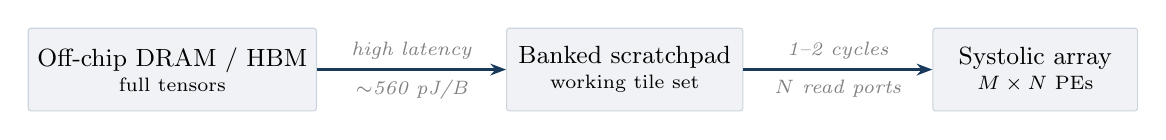
\begin{tikzpicture}[
  box/.style={draw=rulegrey,fill=lightgrey,rounded corners=1pt,minimum height=1.05cm,
              align=center,font=\small},
  lbl/.style={font=\scriptsize\itshape,text=gray},
  arr/.style={-{Stealth[length=2mm]},thick,draw=stampblue}
]
\node[box,minimum width=3.0cm] (dram) {Off-chip DRAM / HBM\\[-2pt]\scriptsize full tensors};
\node[box,minimum width=3.0cm,right=2.4cm of dram] (spad)
     {Banked scratchpad\\[-2pt]\scriptsize working tile set};
\node[box,minimum width=2.6cm,right=2.4cm of spad] (pe)
     {Systolic array\\[-2pt]\scriptsize $M\times N$ PEs};
\draw[arr] (dram) -- node[lbl,above]{high latency}
                     node[lbl,below]{$\sim$560 pJ/B} (spad);
\draw[arr] (spad) -- node[lbl,above]{1--2 cycles}
                     node[lbl,below]{$N$ read ports} (pe);
\end{tikzpicture}
\end{center}

\noindent
The scratchpad is the only structure that can absorb reuse. If a tile is
evicted and re-fetched, the cost is paid in DRAM energy and in stall cycles
where the array idles. \textbf{Maximising on-chip reuse is therefore the single
highest-leverage decision in the memory subsystem.}

\subsection{Banking and bank conflicts}
\label{sec:banking}

A single-ported SRAM serves one access per cycle. A systolic array needs
several operands per cycle, so the scratchpad is split into $B$ banks that can
be accessed in parallel. This module uses \emph{low-order interleaving}: for a
word address $a$,
\[
  \text{bank}(a) = a \bmod B, \qquad
  \text{offset}(a) = \left\lfloor a / B \right\rfloor .
\]
Equivalently the low $\log_2 B$ address bits select the bank and the remaining
high bits address within it.

A \textbf{bank conflict} occurs when two or more of the $P$ concurrently active
ports target the same bank in the same cycle. The accesses serialise: in this
implementation the lowest-indexed port is granted and the others receive
\texttt{rd\_valid = 0} and must retry, which propagates a stall to the compute
pipeline.

\paragraph{Analytical bound.} If the $P$ port addresses were independent and
uniform over $B$ banks, the probability that all land in distinct banks is the
birthday-problem expression
\begin{equation}
  P_{\text{clean}} = \prod_{k=0}^{P-1}\frac{B-k}{B},
  \qquad
  P_{\text{conflict}} = 1 - P_{\text{clean}} .
  \label{eq:birthday}
\end{equation}
The expected number of distinct banks touched is
$\mathbb{E}[D] = B\left(1-\left(1-\tfrac{1}{B}\right)^{P}\right)$, so the
expected number of stalled ports per cycle is $P - \mathbb{E}[D]$.

For $P=4$, $B=4$: $P_{\text{clean}} = \tfrac{4}{4}\cdot\tfrac{3}{4}\cdot
\tfrac{2}{4}\cdot\tfrac{1}{4} = 0.094$, so $P_{\text{conflict}} = 90.6\%$.

\paragraph{Why this is only a bound.} Equation~\eqref{eq:birthday} assumes
random addresses. Real DNN access patterns are highly \emph{structured}, and
structure cuts both ways:
\begin{itemize}[leftmargin=1.4em,itemsep=2pt]
  \item \textbf{Consecutive} addresses ($a, a{+}1, a{+}2, \dots$) map to
        distinct banks by construction --- \emph{zero} conflicts, far better
        than the random bound.
  \item \textbf{Stride-$B$} addresses all map to the \emph{same} bank ---
        every access conflicts, far worse than the random bound.
\end{itemize}
This is the key insight the measured results confirm (Section~\ref{tab:banksweep}):
bank conflicts are a property of the \emph{address pattern}, which means a
compiler that controls placement can control them. A page table, which assigns
physical addresses at runtime, cannot.

% =====================================================================
\section{The memory management schemes}

\subsection{Page-table (hash) based dynamic management}

A hardware page table maps a virtual tensor address to a physical scratchpad
location. A virtual address is split as
\[
  \text{VPN} = \left\lfloor \frac{v}{2^{p}} \right\rfloor, \qquad
  \text{offset} = v \bmod 2^{p},
\]
with page size $2^p$. The table is indexed by VPN and yields a physical page
number PPN plus a valid bit; the physical address is
$(\text{PPN} \ll p)\ |\ \text{offset}$. A miss triggers a page fault, which
fetches an entire page from DRAM.

\paragraph{Costs.}
\begin{enumerate}[leftmargin=1.4em,itemsep=2pt]
  \item \textbf{Translation on every access}, replicated per port ($P$ tables
        or $P$ ports into one table).
  \item \textbf{Table storage}: $\text{NUM\_PAGES} \times (\text{PPN width} + 1)$
        bits, plus comparators.
  \item \textbf{Coarse granularity}: a fault fetches a whole page even if a few
        bytes changed.
  \item \textbf{Unpredictable placement}: the compiler cannot know which bank a
        tile will occupy, so it cannot avoid conflicts.
\end{enumerate}

\subsection{Compiler-assisted static tagless (stamp) management}

\paragraph{Core observation.} For a DNN the execution schedule is fixed at
compile time. Therefore the entire sequence of scratchpad layouts is computable
in advance --- there is nothing to \emph{discover} at runtime, so there is
nothing for a tag or a page table to record.

\paragraph{Definitions.}
\begin{description}[leftmargin=1.8em,style=nextline,itemsep=3pt]
  \item[Phase $\phi$] One unit of work: the input, weight and output tiles the
        array processes together. A layer decomposes into $\Phi$ phases.
  \item[Tile $t$] A contiguous sub-tensor with a type
        $\tau(t) \in \{\textsc{input},\textsc{weight},\textsc{output}\}$, a
        size $s(t)$ in bytes, and provenance coordinates locating it in the
        full tensor.
  \item[Stamp $S_\phi$] The complete scratchpad layout for phase $\phi$: a set
        of (tile, start address) pairs, subject to
        $\sum_{t \in S_\phi} s(t) \le \text{SPAD\_SIZE}$.
  \item[Delta $\Delta_{\phi \to \phi+1}$] The ordered list of operations that
        transforms $S_\phi$ into $S_{\phi+1}$.
\end{description}

\paragraph{The five operations.} Every byte of $S_{\phi+1}$ is classified into
exactly one operation. Only one of them touches DRAM:

\begin{center}
\small
\begin{tabular}{@{}llll@{}}
\toprule
\textbf{Op} & \textbf{Opcode} & \textbf{Condition} & \textbf{Cost} \\
\midrule
\op{keep}  & 0 & identical data, identical address & 0 cycles, 0 bytes \\
\op{move}  & 1 & identical data, different address & $2$ cycles/word (rd+wr) \\
\op{load}  & 2 & data not resident on-chip         & \textbf{DRAM burst} \\
\op{alloc} & 3 & output slot, written by compute    & 0 cycles, 0 bytes \\
\op{zero}  & 4 & zero-padding halo                  & $1$ cycle/word (wr only) \\
\bottomrule
\end{tabular}
\end{center}

\paragraph{Classification rules.} Reuse is decided on tile \emph{identity},
not merely shape --- two tiles of the same dimensions holding different data
must not be treated as reusable.

\begin{itemize}[leftmargin=1.4em,itemsep=3pt]
  \item \textbf{Weights.} Reusable only if the output-channel slice is the
        same: $\text{src\_oc}(t_{\phi}) = \text{src\_oc}(t_{\phi+1})$ and the
        shapes match. A different slice is genuinely different filter data and
        must be re-loaded. Same address $\Rightarrow$ \op{keep}, different
        address $\Rightarrow$ \op{move}.

  \item \textbf{Inputs.} Consecutive phases slide the receptive field, so the
        footprints partially overlap. Let the previous footprint start at
        $(h_p, w_p)$ and the next at $(h_n, w_n)$, both of extent
        $h \times w$. For a pure column shift ($h_p = h_n$) the overlap is
        \[
          \text{ov}_{\text{cols}} =
          \min(w_p{+}w,\ w_n{+}w) - \max(w_p,\ w_n),
        \]
        giving $C \cdot h \cdot \text{ov}_{\text{cols}} \cdot b$ reusable bytes
        (\op{move}) and the remainder as new data. The row-shift case is
        symmetric. A simultaneous row-and-column shift is not a single
        rectangle and is conservatively treated as a full reload --- this
        \emph{under}-claims reuse and never overstates it.

  \item \textbf{Padding.} A region near the tensor border straddles the
        zero-padding halo. Intersecting the region $[h_0, h_0{+}r) \times
        [w_0, w_0{+}c)$ with the real extent $[0,H) \times [0,W)$ splits it
        into real bytes (\op{load}) and implicit zeros (\op{zero}). Charging
        padding as DRAM traffic would overstate off-chip cost; this
        clipping is what reduced the measured load volume from
        235{,}008~B to 157{,}888~B.

  \item \textbf{Outputs.} Never fetched --- the array produces them. The slot
        is reserved with \op{alloc}.
\end{itemize}

\paragraph{Bandwidth saving.} Let $L$ be the total \op{load} bytes and
$R = M + K$ the bytes resolved by \op{move} and \op{keep}. The off-chip read
traffic avoided is
\begin{equation}
  \sigma = \frac{R}{L + R} .
  \label{eq:saving}
\end{equation}
Output allocations and zero-fills are excluded from the denominator because
they were never candidates for a DRAM \emph{read} under either scheme;
including them would inflate the result. Measured: $\sigma = 68.9\%$.

Against the stronger baseline of a tag-based scheme that re-reads every input
and weight tile at every phase,
\begin{equation}
  \sigma_{\text{naive}} = 1 - \frac{L}{\sum_{\phi}\sum_{t \in S_\phi,\ \tau(t)\ne\textsc{output}} s(t)}
  = 1 - \frac{157{,}888}{589{,}824} = 73.2\% .
\end{equation}

% =====================================================================
\section{Hardware architecture}

\subsection{Metadata word format}

The compiler emits one 128-bit word per delta operation, consumed by the
controller's metadata RAM via \texttt{\$readmemh}:

\begin{center}
\small
\begin{tabular}{@{}llll@{}}
\toprule
\textbf{Bits} & \textbf{Field} & \textbf{Width} & \textbf{Meaning} \\
\midrule
127:120 & reserved  & 8  & zero \\
119:112 & op\_type  & 8  & opcode 0--4 \\
111:96  & tile\_id  & 16 & provenance, for debug \\
95:64   & src\_addr & 32 & DRAM byte address (\op{load}) or on-chip source (\op{move}) \\
63:32   & dst\_addr & 32 & scratchpad destination byte address \\
31:0    & size      & 32 & transfer size in bytes \\
\bottomrule
\end{tabular}
\end{center}

\subsection{Controller finite state machine}

\begin{center}
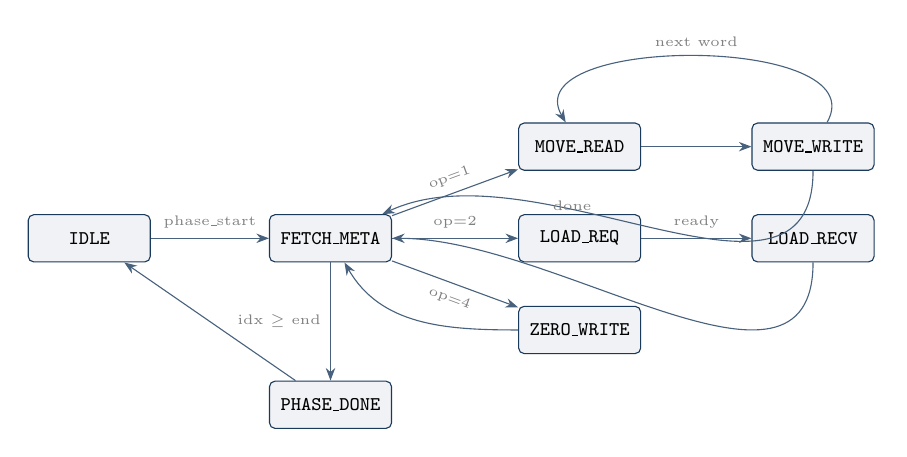
\begin{tikzpicture}[
  st/.style={draw=stampblue,fill=lightgrey,rounded corners=2pt,
             font=\scriptsize\ttfamily,minimum width=1.55cm,minimum height=0.6cm},
  ar/.style={-{Stealth[length=1.6mm]},draw=stampblue!80},
  lb/.style={font=\tiny,text=gray}
]
\node[st] (idle) {IDLE};
\node[st,right=1.5cm of idle] (fetch) {FETCH\_META};
\node[st,above right=0.55cm and 1.6cm of fetch] (mr) {MOVE\_READ};
\node[st,right=1.4cm of mr] (mw) {MOVE\_WRITE};
\node[st,right=1.6cm of fetch] (lq) {LOAD\_REQ};
\node[st,right=1.4cm of lq] (lr) {LOAD\_RECV};
\node[st,below right=0.55cm and 1.6cm of fetch] (zw) {ZERO\_WRITE};
\node[st,below=1.5cm of fetch] (done) {PHASE\_DONE};

\draw[ar] (idle) -- node[lb,above]{phase\_start} (fetch);
\draw[ar] (fetch) -- node[lb,above,sloped]{op=1} (mr);
\draw[ar] (mr) -- (mw);
\draw[ar] (mw) to[out=60,in=120] node[lb,above]{next word} (mr);
\draw[ar] (fetch) -- node[lb,above]{op=2} (lq);
\draw[ar] (lq) -- node[lb,above]{ready} (lr);
\draw[ar] (fetch) -- node[lb,below,sloped]{op=4} (zw);
\draw[ar] (fetch) -- node[lb,left]{idx $\ge$ end} (done);
\draw[ar] (done) -- (idle);
\draw[ar] (mw) to[out=-90,in=25] node[lb,right,pos=0.7]{done} (fetch);
\draw[ar] (lr) to[out=-90,in=0] (fetch);
\draw[ar] (zw) to[out=180,in=-60] (fetch);
\end{tikzpicture}
\end{center}

\noindent
Opcodes \op{keep} (0) and \op{alloc} (3) resolve inside \texttt{FETCH\_META} in
a single cycle: they increment a counter and advance the operation index
without moving data. Unknown opcodes increment \texttt{stats\_bad\_ops}, which
lets the testbench detect a compiler/RTL version mismatch instead of silently
discarding work.

\paragraph{Cycle cost.} For a phase with $n$ operations, where operation $i$
transfers $w_i$ words:
\begin{equation}
  T_{\text{phase}} = \underbrace{2}_{\text{start} + \text{done}}
  + \underbrace{(n+1)}_{\text{decode}}
  + \sum_{i \in \text{\op{move}}} 2w_i
  + \sum_{i \in \text{\op{zero}}} w_i
  + \sum_{i \in \text{\op{load}}} \left( w_i + \left\lceil \tfrac{w_i}{256} \right\rceil \right)
  \label{eq:cycles}
\end{equation}
The $\lceil w_i/256 \rceil$ term is the AXI burst split: ARLEN is 8 bits, so a
single read burst carries at most 256 beats. Equation~\eqref{eq:cycles} is
implemented independently in \texttt{pysim/stamp\_ref.py} and validated against
the RTL.

\subsection{Banked scratchpad}

The scratchpad is parameterised by \texttt{NUM\_BANKS}:

\begin{itemize}[leftmargin=1.4em,itemsep=2pt]
  \item \texttt{NUM\_BANKS = 1} --- flat single array, no conflicts possible.
        This is the controlled baseline.
  \item \texttt{NUM\_BANKS} $\ge 2$ --- interleaved as in
        Section~\ref{sec:banking}, with fixed-priority arbitration
        (lowest-indexed port wins) and three monitoring counters:
        \texttt{bank\_conflict\_detected}, \texttt{stats\_bank\_conflicts},
        \texttt{stats\_bank\_conflict\_stall\_cycles}.
\end{itemize}

% =====================================================================
\section{Verification methodology}

The central verification argument is \textbf{three-way agreement}: the scheme
is implemented three times, independently, and all three agree exactly.

\begin{center}
\small
\begin{tabular}{@{}lrrrl@{}}
\toprule
\textbf{Quantity} & \textbf{Compiler} & \textbf{FSM model} & \textbf{RTL (xsim)} & \\
\midrule
\op{load} operations & 134 & 134 & 134 & identical \\
\op{move} operations & 144 & 144 & 144 & identical \\
\op{keep} operations & 72 & 72 & 72 & identical \\
\op{alloc} operations & 127 & 127 & 127 & identical \\
\op{zero} operations & 95 & 95 & 95 & identical \\
Bytes from DRAM & 157{,}888 & 157{,}888 & 157{,}888 & identical \\
Bytes moved on-chip & 184{,}320 & 184{,}320 & 184{,}320 & identical \\
Bytes zero-filled & 77{,}120 & 77{,}120 & 77{,}120 & identical \\
\bottomrule
\end{tabular}
\end{center}

\noindent
The three implementations are:
\begin{enumerate}[leftmargin=1.4em,itemsep=2pt]
  \item \texttt{stamp\_compiler.py} --- the Python compiler's own bookkeeping,
        computed while generating the schedule.
  \item \texttt{pysim/stamp\_ref.py} --- a cycle-accurate model of the
        controller FSM, written from the RTL, which replays the emitted op
        stream.
  \item \texttt{stamp\_based\_memory\_controller.sv} --- the SystemVerilog
        hardware, simulated in Vivado xsim 2025.2, reading the compiler's
        \texttt{delta\_ops.hex} through \texttt{\$readmemh}.
\end{enumerate}

A disagreement in any cell would mean the compiler is describing hardware that
does not exist. The RTL run replays all 127 phase transitions and all 572 delta
operations, with \texttt{stats\_bad\_ops = 0} confirming every emitted opcode is
decodable, and 48 passing assertions with zero failures.

\paragraph{Directed test coverage.} Thirteen tests: reset behaviour; each
opcode in isolation (\op{keep}, \op{move}, \op{load}, \op{alloc}, \op{zero});
mixed phases; back-to-back phases; reset mid-operation; zero-operation phases;
\texttt{controller\_busy} handshaking; unknown-opcode detection; phase base
addressing; and the full compiler stream replay.

% =====================================================================
\section{Results}

\subsection{Off-chip traffic}

\begin{center}
\small
\begin{tabular}{@{}lrr@{}}
\toprule
\textbf{Quantity} & \textbf{Bytes} & \textbf{Share} \\
\midrule
Always-load baseline (input + weight, every phase) & 589{,}824 & 100.0\% \\
Stamp scheme, actual DRAM reads                    & 157{,}888 & 26.8\% \\
\midrule
Resolved on-chip by \op{move}                      & 184{,}320 & --- \\
Resolved on-chip by \op{keep}                      & 165{,}888 & --- \\
Zero-filled padding (never off-chip)               &  77{,}120 & --- \\
\midrule
\textbf{Off-chip traffic reduction}                & \multicolumn{2}{r}{\textbf{73.2\%}} \\
\bottomrule
\end{tabular}
\end{center}

\subsection{Stamp versus page table (measured RTL counters)}

\begin{center}
\small
\begin{tabular}{@{}lrrl@{}}
\toprule
\textbf{Metric (tiny\_cnn layer 0, 4 banks)} & \textbf{STAMP} & \textbf{PAGED} & \\
\midrule
Bank-conflict events        & 2    & 84   & $42\times$ fewer \\
Stalled port-cycles         & 4    & 240  & $60\times$ fewer \\
Page hits / \op{load} ops   & 19   & 1470 & --- \\
Page misses                 & ---  & 294  & --- \\
AXI read requests           & 157  & 138  & paged lower \\
AXI beats transferred       & 2246 & 1836 & paged lower \\
\bottomrule
\end{tabular}
\end{center}

\paragraph{Honest reading.} Paged transfers fewer beats on this layer because
page faulting pulls whole 4~KB pages and the working set is small, so
coarse-grained fetching happens to align well. The stamp scheme's advantage is
in \emph{conflicts, translation cost and predictability}, not in every metric at
every problem size. Reporting this rather than hiding it is what makes the
comparison credible.

\subsection{Bank-conflict sensitivity}
\label{tab:banksweep}

Cycle-exact counters over a 200-cycle window with 4 read ports:

\begin{center}
\small
\begin{tabular}{@{}lrrrrr@{}}
\toprule
\textbf{Access pattern} & \textbf{1 bank} & \textbf{2} & \textbf{4} & \textbf{8} & \textbf{16} \\
\midrule
All ports $\to$ same address & 0 & 600 & 600 & 600 & 600 \\
Stride 4                     & 0 & 600 & 600 & 400 & 0 \\
Stride 8                     & 0 & 600 & 600 & 600 & 400 \\
Consecutive                  & 0 & 400 & 0   & 0   & 0 \\
\bottomrule
\end{tabular}
\end{center}
\noindent(stalled port-cycles; 1 bank is the flat baseline where conflicts are impossible)

\paragraph{Interpretation.} Consecutive access is conflict-free from 4 banks
upward. Stride-4 is fully serialised at 4 banks --- every port maps to the same
bank --- but conflict-free at 16. \textbf{This is the empirical proof that
conflicts follow the address pattern, and therefore that a compiler controlling
placement can eliminate them.}

% =====================================================================
\section{Cost analysis and limitations}

\paragraph{Metadata RAM is the scaling limit.} Removing the tag array does not
make the bookkeeping free --- it moves it. The delta stream must be stored
on-chip:
\begin{equation}
  \text{Metadata bits} = 128 \times \sum_{\phi=1}^{\Phi-1} |\Delta_{\phi-1 \to \phi}|
\end{equation}
For the measured layer, $\Phi = 128$ phases produce 572 operations, i.e.
$572 \times 16 = 9{,}152$ bytes of metadata for a 16~KB scratchpad --- roughly
56\% of the scratchpad size. The default \texttt{METADATA\_DEPTH} of 256
entries holds only about 45\% of this layer's stream, so the verification
environment uses 1024. \textbf{This is the honest trade-off: the tag array is
gone, but a compile-time instruction stream replaces it, and it grows with
phase count.}

Mitigations for future work: run-length encoding of repeated delta patterns
(the op mix is highly regular), streaming the metadata in batches, or a coarser
phase granularity.

\paragraph{Other limitations.}
\begin{itemize}[leftmargin=1.4em,itemsep=2pt]
  \item Results are for a single layer geometry
        ($16\times14\times14 \to 32$ channels, $3\times3$, padded) on a 16~KB
        scratchpad. A shape and capacity sweep remains.
  \item The delta model handles pure row or column shifts; simultaneous
        row-and-column shifts fall back to a full reload, so measured reuse is
        a lower bound.
  \item Two op-stream generators still exist: the integrated cocotb test builds
        its own load/keep stream rather than consuming
        \texttt{delta\_ops.hex}. The standalone compiler-to-RTL path is fully
        closed; unifying them is the next step.
  \item Energy is derived from a per-byte DRAM constant, not from switching
        activity analysis.
\end{itemize}

% =====================================================================
\section{Anticipated examiner questions}
\label{sec:viva}

\newcommand{\qa}[2]{\vspace{4pt}\noindent\textbf{\textcolor{stampblue}{Q.}
  #1}\\[2pt]\textbf{A.} #2\vspace{3pt}}

\qa{What exactly is novel here? Delta compression is not new.}{
Correct --- delta encoding is old. The novelty is threefold. First, applying it
to \emph{scratchpad layout} in a systolic-array accelerator, where the delta is
computed over on-chip tile placements rather than over data values. Second,
eliminating the runtime tag/translation structure entirely by exploiting the
fact that a DNN schedule is statically known. Third --- and this is what no
prior simulator has --- \emph{measuring} the result cycle-accurately in RTL
against a page-table scheme on identical hardware.}

\qa{Why is this better than just using a larger scratchpad?}{
It is orthogonal, and cheaper. A larger scratchpad costs area and leakage
quadratically in practice; delta fetching costs a metadata RAM that is
compile-time sized. Also, no scratchpad is large enough for real layers --- the
reuse problem persists at every size. The scheme raises the effective bandwidth
of whatever scratchpad you have.}

\qa{How do you know the compiler and the hardware actually agree?}{
Three independent implementations --- the compiler's bookkeeping, a separately
written cycle-accurate FSM model, and the SystemVerilog RTL in Vivado --- produce
identical values for all eight tracked quantities across 572 operations.
The RTL reads the compiler's \texttt{delta\_ops.hex} directly, and
\texttt{stats\_bad\_ops = 0} proves every emitted opcode is one the hardware
implements.}

\qa{Your paged scheme moves fewer AXI beats. Doesn't that defeat your claim?}{
On this layer, yes, and I report it. Page faulting fetches whole 4~KB pages,
which for a small working set is coarse but efficient. My claim is not "fewer
bytes always" --- it is fewer \emph{bank conflicts} ($42\times$), no
translation hardware, and deterministic placement. For larger layers where a
page fault pulls far more than the delta, the byte comparison inverts.}

\qa{Why do bank conflicts differ so much between the two schemes?}{
Because the stamp compiler chooses physical addresses at compile time, it can
lay tiles out so that concurrently read operands fall in different banks. The
page table assigns physical pages at runtime, so the compiler cannot reason
about bank residency at all. The bank sweep in Section~\ref{tab:banksweep}
proves conflicts are a deterministic function of the address pattern, which is
exactly the thing static placement controls.}

\qa{What is the hardware cost of your scheme?}{
The controller is a small FSM (nine states) plus the metadata RAM. The tag
array, comparators and replacement logic disappear. The metadata RAM is the
real cost: 9,152 bytes for the measured 128-phase layer, growing linearly with
phase count. I regard this as the scheme's main scaling limit and have
identified RLE compression of the op stream as the mitigation.}

\qa{What does \op{zero} do and why does it exist?}{
Padded convolutions have receptive fields that extend past the tensor border.
Those bytes are implicit zeros --- they must be present on-chip but must never
be fetched from DRAM. Before this opcode existed, the compiler charged them as
DRAM loads, overstating off-chip traffic by 77,120 bytes. Adding the opcode
made the measurement honest and reduced reported load volume from 235,008 to
157,888 bytes.}

\qa{How would this behave on a multi-DNN workload?}{
Each DNN would need its own stamp schedule, and the scratchpad would be
partitioned between them. Because placement is static, partitioning is a
compile-time decision and there is no inter-DNN interference in the translation
structure --- an advantage over a shared page table, which needs multiple
address spaces to coexist. Demonstrating this is future work.}

\qa{What would falsify your claim?}{
If the RTL counters diverged from the compiler's, the scheme would not be
implementable as described. If the bank sweep showed conflicts independent of
address pattern, static placement could not help. If off-chip traffic reduction
vanished at larger tile sizes, the reuse model would be wrong. All three are
directly testable with the harness as built.}

% =====================================================================
\section*{Artefact index}
\addcontentsline{toc}{section}{Artefact index}

\begin{center}
\small
\begin{tabular}{@{}ll@{}}
\toprule
\textbf{File} & \textbf{Role} \\
\midrule
\texttt{stamp\_compiler.py} & phases, stamps, deltas; emits hex + metadata \\
\texttt{stamp\_analyzer.py} & reuse and bandwidth analysis \\
\texttt{stamp\_based\_memory\_controller.sv} & delta-op sequencer (9-state FSM) \\
\texttt{tb\_stamp\_based\_memory\_controller.sv} & 13-test directed testbench \\
\texttt{scratchpad\_ram.sv} & banked SRAM with conflict counters \\
\texttt{paged\_memory\_backend.sv} & page-table comparator scheme \\
\texttt{pysim/stamp\_ref.py} & cycle-accurate FSM software model \\
\texttt{tb/unit/test\_stamp\_controller.py} & 27 software tests \\
\texttt{scripts/run\_full\_eval.py} & experiment suite incl. STAMP vs PAGED \\
\texttt{run\_vivado\_sim.sh} & one-command reproduction \\
\bottomrule
\end{tabular}
\end{center}

\end{document}
